\chapter{Problémadefiníció} \label{Problem_def}
Valódi ipari környezetben gyakran előfordulnak olyan esetek, amelyekben a megoldandó problémát nem lehet tisztán determinisztikus paraméterekkel leírni, ezeket felhasználva megoldani, hanem szükség van új, a bizonytalanságokat kifejező, sztochasztikus paraméterekre is.
Változó piaci környezetben ilyen sztochasztikus paraméternek számítanak például a termék iránti kereslet, illetve a piaci ár, amin a terméket értékesíteni lehet.
Belátható az is, hogy ezek a paraméterek sokban befolyásolják a maximalizálandó profitot.
Vegyünk például egy olyan esetet, amelyben a keresletnél többet termeltünk, ez esetben a keletkező többletet nem tudjuk értékesíteni, ez akár további kiadásokkal is járhat a többlet termék esetleges tárolási költsége miatt, ezeket a kiadásokat túltermelési költségeknek nevezzük.
Beszélhetünk alul termelési költségről is, például abban az esetben, ha egy szerződésben foglalt elvárt darabszám legyártásának teljesítése nem következett be, ebben az esetben akár kötbért fizetésére is kötelezhető lehet adott cég.
Ezek alapján egy lehetséges profit függvény szemléltetésére szolgál a \ref{profit_func}. ábra.
\begin{figure}
\begin{center}
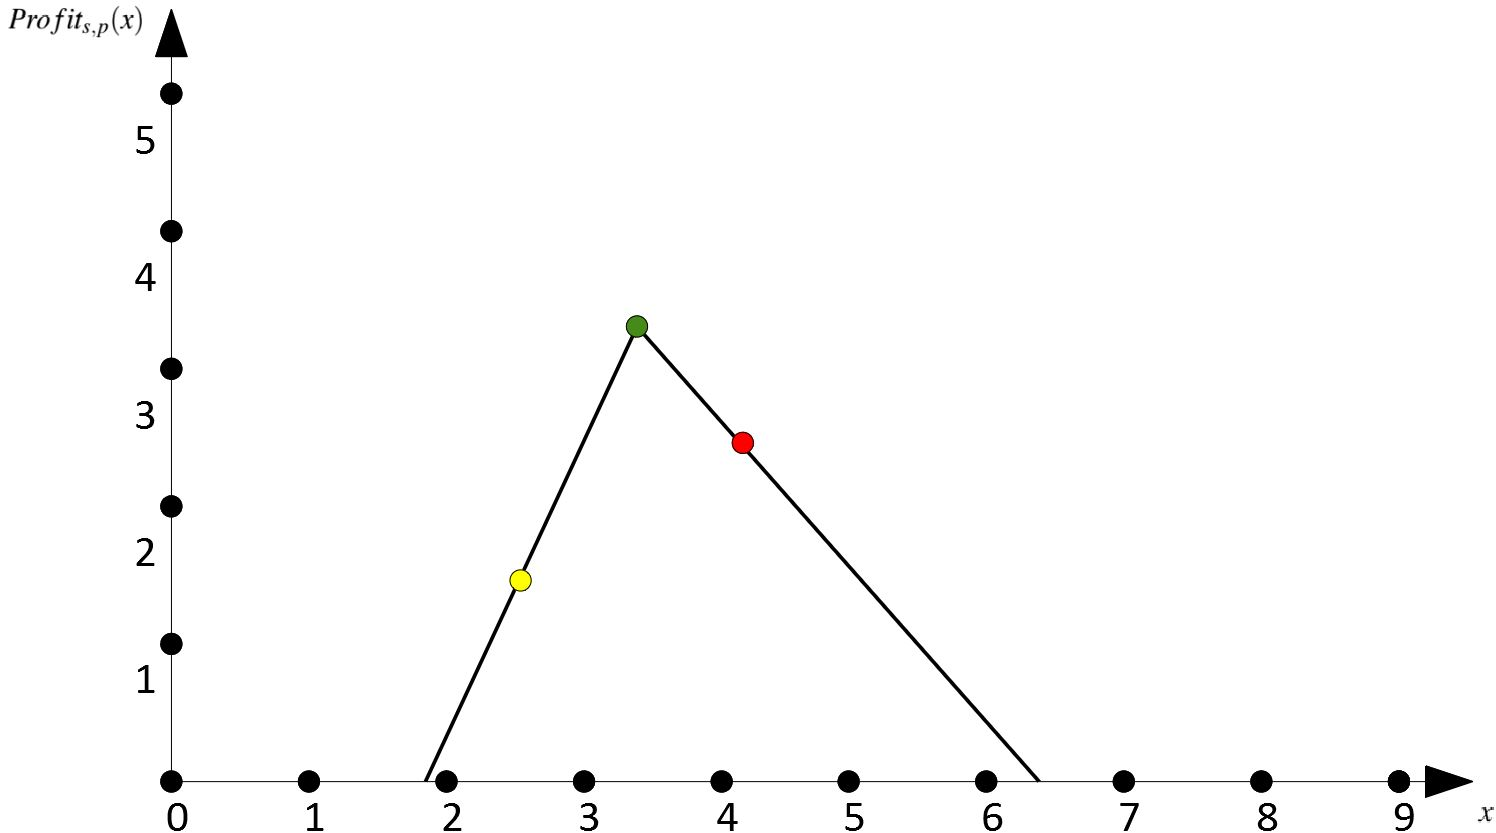
\includegraphics[scale=0.38]{profitFunc}
\caption{A profit függvény szemléltetése}
\label{profit_func}
\end{center}
\end{figure}
Az ábra alapján jól látszik, hogy adott termék bevétele akkor lesz maximális, ha a kereslettel egyező darabszámot gyártunk az adott termékből (zöld pont a \ref{profit_func}. ábrán), ha ennél kevesebbet gyártunk a termékből, akkor a kereslet kielégítéséből eredő profit is elmarad, illetve további többlet költség kerül levonásra a profit összegéből az esetleges alul termelési plusz költségek miatt (pl. sárga pont a \ref{profit_func}. ábrán), abban az esetben pedig, ha a keresletet meghaladó mennyiséget gyártunk adott termékből, a kereslet kielégítődik ugyan, és bevételünk maximális lenne az adott piaci keresletet figyelembe véve, azonban a túltermelés következtében létrejött többlet tárolási költségét le kell vonjuk a profit értékéből (pl. piros pont a \ref{profit_func}. ábrán) \footnote{Előfordulhat olyan eset, amelyben az alul-, és túltermelési költségekkel nem kell számolni, ebben az esetben a kereslet értékének eléréséig a profit a termelt mennyiséggel arányosan lineárisan növekedni fog, majd onnantól kezdve konstans módon beáll a maximális értékre, ugyanis a felesleg értékesítése nem lehetséges, ha arra nincs kereslet, viszont annak tárolás nem okoz plusz költséget.}.
Arra kell törekedni tehát, hogy a lehetőségeket mérlegelve minden termékből annyit gyártsunk, hogy az, az adott forgatókönyvben szereplő keresletet kielégítse, vagy azt a legkedvezőbb módon megközelítse valamelyik irányból, ügyelve az alul-, és túltermelési költségekre.
Jól látható, hogy az ilyen fajta problémák merőben eltérőek, az eredeti determinisztikus problémákhoz képest, éppen ezért egy új módszer kidolgozása szükséges ezek megoldásához.
Extrém esetekben előállhat olyan helyzet is, hogy a rendelkezésre álló determinisztikus paraméterek (pl. gépek száma), az aktuális időhorizont, illetve a sztochasztikus paraméterek aktuális értéke miatt a profit függvény $x$-ben felvett értéke negatív szám lesz, ez esetben inkább a veszteségek minimalizálásáról beszélhetünk, mintsem profit maximalizálásról, az új módszerek kidolgozása során fel kell tehát ilyen esetekre is készülni.
\pagebreak

A megoldandó problémák a sztochasztikus esetben is a determinisztikus throughput maximalizálásnál használt paraméterekkel adottak, pl.: minden terméket a receptje azonosít be, ezen kívül adott a termékek előállítására használható berendezések halmaza, illetve a termelésre rendelkezésre álló időhorizont.
Az determinisztikus paramétereken kívül azonban sztochasztikus esetben különböző bizonytalanságot kifejező paraméterek is adottak minden termékre, amelyek valószínűségeit különböző scenariokba, forgatókönyvekbe csoportosítjuk.
Ezáltal minden forgatókönyvre adott: 
\begin{itemize}
\item{A forgatókönyv valószínűsége}
\item{A termék ára (1 batch ára) az adott forgatókönyvben}
\item{A termék iránti kereslet az adott forgatókönyvben}
\item{A túltermelés, és az alul termelés költsége az adott forgatókönyvben}
\end{itemize}
A cél az, hogy döntést hozzunk a termelt batch-ek darabszámát, illetve egyes esetekben azok méretét illetően, miközben egy olyan kivitelezhető ütemtervet biztosítunk, amelyet követve maximális várható profitot érhetünk el.
\section{A különböző feladat osztályok} \label{problem_csop}
A batch méretekkel kapcsolatos döntések alapján 3 eset különböztethető meg:
\begin{itemize}
\item \textbf{Preventív ütemezés kötött batch mérettel} Ebben az esetben minden termékhez adott egy batch méret, az egyetlen preventív döntés amit hoznunk kell, hogy hány darab batch-et gyártunk az adott termékből.
\item \textbf{Preventív ütemezés változó batch mérettel} Ebben az esetben nem csak a batch darabszám ,de annak a mérete is kiválasztható, de csak preventív módon a bizonytalan események bekövetkezése előtt.
\item \textbf{Két lépcsős ütemezés (two stage)} Ebben az esetben a batch darabszámot előre ki kell választanunk, azonban annak a méretéről a bizonytalan események bekövetkezése után is döntést hozhatunk.
\end{itemize}
Kezdetben feltételezzük, hogy a receptek és a termékek között 1-1 kapcsolat van, azaz egy recept sem eredményez több terméket, illetve egyetlen termék sem állítható elő több fajta recepttel.
Az \ref{extended_multiproduct}. pontban azonban kitérek azokra az esetekre, amelyekben ez a feltételezés nem állja meg a helyét.
\section{A probléma formális bemenete} \label{problem_parameters}
A \ref{problem_csop}. alfejezetben bevezetett sztochasztikus esetek kezeléséhez az determinisztikus throughput maximalizáló algoritmus jelentős része felhasználható változtatások nélkül (vagy csak minimális változtatások árán, lsd. \ref{refactor}. alfejezet).
Az egyetlen meghatározó különbség az un. "revenue" függvényben figyelhető meg, amely célja, hogy az adott konfigurációra nézve kiszámítsa a várható profitot.
A probléma megoldása során használt paraméterek jelölései:
\begin {description}
\item[$P$]  a termékek halmaza
\item[$b_p$]  a legyártott batch-ek darabszáma az adott konfigurációban
\item[$s_p$]  a termék batch mérete (fix batch méret esetén) [Kg]
\item[$s_p^{min},s_p^{max}$]  adott termékhez tartozó lehetséges legkisebb, legnagyobb batch méret (válzotó batch méret esetén) [Kg]
\item[$S$]  a forgatókönyvek halmaza
\item[$prob_s$]  s forgatókönyv valószínűsége $s	\in S$
\item[$dem_{s,p}$]  p termék iránti kereslet az s forgatókönyvben $s	\in S, p	\in P$ [Kg]
\item[$price_{s,p}$]  p termék ára az s forgatókönyvben $s	\in S, p	\in P$ [Cost Unit/Kg]
\item[$oc_{s,p}, uc_{s,p}$]  p termék túl-, és alul termelési költsége s forgatókönyvben $s	\in S, p	\in P$ [Cost Unit/Kg]
\end {description}